\chapter{Introduction}

\TODO{what is a critical system, how it is different}

In critical systems such as airplanes and cars, it is important that tasks running on the hardware meet their deadlines. For example, in a car's braking system, missing a program deadline can lead to loss of control over the vehicle. Therefore, it is crucial to have a rigorous analysis that can provide an upper bound for the program's execution time on a given hardware platform. In non-critical real-time applications, the execution time bound can be estimated by measuring the execution time for many input values. This gives the maximum observed execution time, which usually underestimates the real \textit{worst-case execution time (WCET)}.

In critical real-time systems, this approach is not enough because some cases may be missed during observation, as shown in Figure \ref{fig:timing-distribution}. The real WCET can only be found by testing the program on all possible inputs, which is usually not possible due to the large number of cases. Therefore, methods to estimate WCET bounds use abstractions of the program and hardware. These methods may overestimate the WCET because of simplifications, but they are more scalable.

\begin{figure}[H]
    \centering
    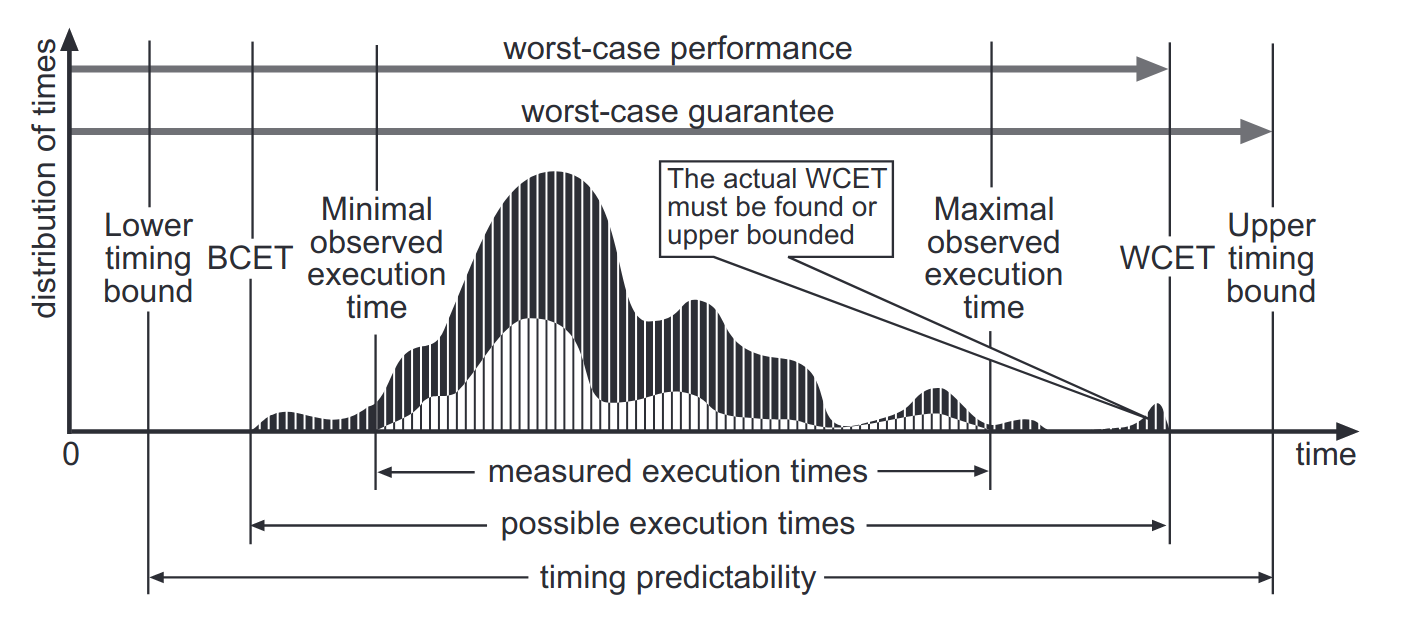
\includegraphics[width=\textwidth]{figures/timing-distribution.png}
    \caption{Timing analysis notations. The lower curve shows a subset of measured executions. The darker curve, an envelope of the former, shows the times of all executions (from \cite{ferdinand_worst_2004}).}
    \label{fig:timing-distribution}
\end{figure}

Usually, WCET analysis is divided into several phases, each focusing on a part of the hardware or software. For example, in the software part, memory analysis assigns address bounds for each instruction \cite{Harrison_Ranges_1977}, and loop bounds analysis finds the bounds for loop iterations as constants or formulas \cite{Healy_bounding_1998}. On the hardware side, there are analyzes for cache, main memory access latency, and pipeline. Together, these analyzes help to find the longest path of a program, which gives the WCET bound.

\begin{figure}
    \centering
    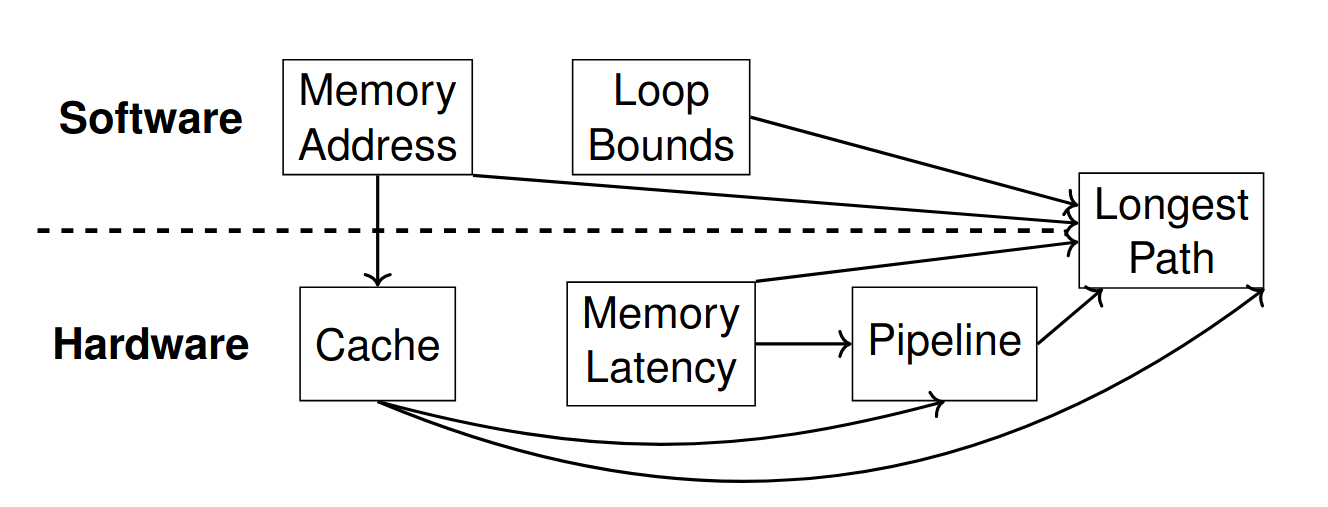
\includegraphics[width=0.7\textwidth]{figures/wcet-deps.png}
    \caption{WCET analysis phases and their dependencies. (\TODO{Image source})}
    \label{fig:wcet-deps}
\end{figure}

Dividing WCET analysis into phases creates the phase ordering problem: one phase may need information from another. Sometimes, these dependencies are circular. For example, in Out-of-Order (OoO) processors, the instruction order depends on the architecture state, which also affects cache access. This means cache analysis needs pipeline analysis. For timing analysis, it is desirable to have composable systems \cite{Puschner_computing_1997}.

However, most architectures are not composable and have so-called \textit{timing anomalies (TA)}. A TA happens when local worst cases do not lead to a global worst case. TAs are seen in pairs of execution traces where the initial hardware state is different, but the instruction sequences are the same. Different cache states can cause variations in timing because of a miss in one trace and a hit in another.

\begin{example}
Figure \ref{fig:TA1} shows an example of such an anomaly. The assembly sequence has 4 instructions ($A,B,C,D$) with data dependencies $A \rightarrow B$ and $C \rightarrow D$. Figure \ref{fig:TA1-trace} shows two traces ($\alpha, \beta$) from running the program. There is a difference in the latency of instruction $A$ ($1$ in $\alpha$ and $2$ in $\beta$). In trace $\alpha$, the variation seems better, but the total execution time is higher, which shows an anomaly.
\label{ex:simple-ta}
\end{example}

\begin{figure}[H]
    \centering
    \begin{subfigure}[t]{0.3\textwidth}
        \centering
        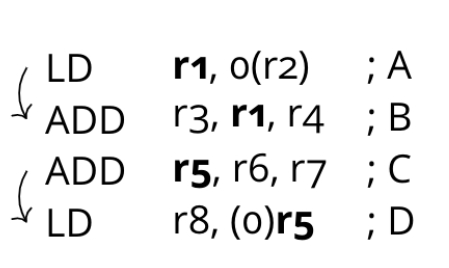
\includegraphics[width=\textwidth]{figures/first-TA-ex-input.png}
        \caption{Input assembly sequence}
        \label{fig:TA1-code}
    \end{subfigure}
    \hfill
    \begin{subfigure}[t]{0.5\textwidth}
        \centering
        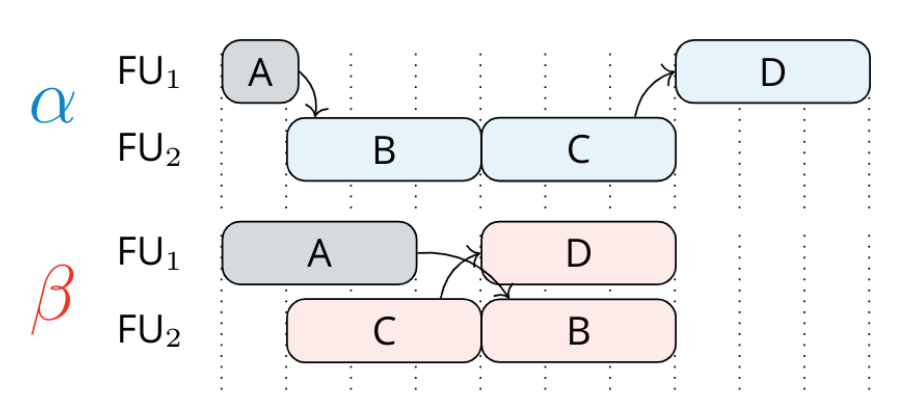
\includegraphics[width=\textwidth]{figures/first-TA-ex-trace.png}
        \caption{Scheduling on functional units comparison}
        \label{fig:TA1-trace}
    \end{subfigure}
    \caption{TA caused by variation in latency of instruction \textit{A} (from \cite{binder_definitions_2022})}
    \label{fig:TA1}
\end{figure}

Timing anomalies are a serious problem for timing predictability. Understanding their nature is important to estimate their impact on global execution time or to design hardware without TAs. Many hardware features can cause TAs, such as caches and memory buses. In this work, we focus on branch prediction. We start by explaining the microarchitecture context, then review existing definitions, and finally present our framework to find branch-related TAs and propose a formal definition for them.
